\documentclass[12pt]{article} 
% \documentclass[12pt]{amsart} 

% Custom definitions
% To use this customization file, insert the line "% Custom definitions
% To use this customization file, insert the line "% Custom definitions
% To use this customization file, insert the line "\input{custom}" in the header of the tex file.

% Formatting

\tolerance=1000
\usepackage[margin=1in]{geometry}


% Packages

% \usepackage{amssymb,latexsym}
\usepackage{amssymb,amsfonts,amsmath,latexsym,amsthm}
\usepackage[usenames,dvipsnames]{color}
\usepackage[]{graphicx}
\usepackage[space]{grffile}
\usepackage{mathrsfs}   % fancy math font
% \usepackage[font=small,skip=0pt]{caption}
\usepackage[skip=0pt]{caption}
\usepackage{subcaption}
\usepackage{verbatim}
\usepackage{url}
\usepackage{bm}
\usepackage{dsfont}
\usepackage{extarrows}
\usepackage{multirow}
% \usepackage{wrapfig}
% \usepackage{epstopdf}
\usepackage{rotating}
\usepackage{tikz}
\usetikzlibrary{fit}					% fitting shapes to coordinates
%\usetikzlibrary{backgrounds}	% drawing the background after the foreground

\usepackage{fancyhdr}

\fancypagestyle{firststyle}{
   \fancyhf{}
   \renewcommand{\footrulewidth}{0.4pt}
   \fancyfoot[L]{\footnotesize This work is licensed under a \href{http://creativecommons.org/licenses/by-nc-nd/4.0/}{Creative Commons BY-NC-ND 4.0 International License}.\\ Jeffrey W. Miller (2015). \textit{Lecture Notes on Bayesian Statistics}. Duke University, Durham, NC.}
}


% \usepackage[dvipdfm,colorlinks,citecolor=blue,linkcolor=blue,urlcolor=blue]{hyperref}
\usepackage[colorlinks,citecolor=blue,linkcolor=blue,urlcolor=blue]{hyperref}
%\usepackage{hyperref}
\usepackage[authoryear,round]{natbib}


%  Theorems, etc.

\theoremstyle{plain}
\newtheorem{theorem}{Theorem}[section]
\newtheorem{corollary}[theorem]{Corollary}
\newtheorem{lemma}[theorem]{Lemma}
\newtheorem{proposition}[theorem]{Proposition}
\newtheorem{condition}[theorem]{Condition}
% \newtheorem{conditions}[theorem]{Conditions}

\theoremstyle{definition}
\newtheorem{definition}[theorem]{Definition}
% \newtheorem*{unnumbered-definition}{Definition}
\newtheorem{example}[theorem]{Example}
\theoremstyle{remark}
\newtheorem*{remark}{Remark}
\numberwithin{equation}{section}



% Document-specific shortcuts
\newcommand{\btheta}{{\bm\theta}}
\newcommand{\bbtheta}{{\pmb{\bm\theta}}}

\newcommand{\commentary}[1]{\ifx\showcommentary\undefined\else \emph{#1}\fi}

\newcommand{\term}[1]{\textit{\textbf{#1}}}

% Math shortcuts

% Probability distributions
\DeclareMathOperator*{\Exp}{Exp}
\DeclareMathOperator*{\TExp}{TExp}
\DeclareMathOperator*{\Bernoulli}{Bernoulli}
\DeclareMathOperator*{\Beta}{Beta}
\DeclareMathOperator*{\Ga}{Gamma}
\DeclareMathOperator*{\TGamma}{TGamma}
\DeclareMathOperator*{\Poisson}{Poisson}
\DeclareMathOperator*{\Binomial}{Binomial}
\DeclareMathOperator*{\NormalGamma}{NormalGamma}
\DeclareMathOperator*{\InvGamma}{InvGamma}
\DeclareMathOperator*{\Cauchy}{Cauchy}
\DeclareMathOperator*{\Uniform}{Uniform}
\DeclareMathOperator*{\Gumbel}{Gumbel}
\DeclareMathOperator*{\Pareto}{Pareto}
\DeclareMathOperator*{\Mono}{Mono}
\DeclareMathOperator*{\Geometric}{Geometric}
\DeclareMathOperator*{\Wishart}{Wishart}

% Math operators
\DeclareMathOperator*{\argmin}{arg\,min}
\DeclareMathOperator*{\argmax}{arg\,max}
\DeclareMathOperator*{\Cov}{Cov}
\DeclareMathOperator*{\diag}{diag}
\DeclareMathOperator*{\median}{median}
\DeclareMathOperator*{\Vol}{Vol}

% Math characters
\newcommand{\R}{\mathbb{R}}
\newcommand{\Z}{\mathbb{Z}}
\newcommand{\E}{\mathbb{E}}
\renewcommand{\Pr}{\mathbb{P}}
\newcommand{\I}{\mathds{1}}
\newcommand{\V}{\mathbb{V}}

\newcommand{\A}{\mathcal{A}}
\newcommand{\C}{\mathcal{C}}
\newcommand{\D}{\mathcal{D}}
\newcommand{\Hcal}{\mathcal{H}}
\newcommand{\M}{\mathcal{M}}
\newcommand{\N}{\mathcal{N}}
\newcommand{\X}{\mathcal{X}}
\newcommand{\Zcal}{\mathcal{Z}}
\renewcommand{\P}{\mathcal{P}}

\newcommand{\T}{\mathtt{T}}
\renewcommand{\emptyset}{\varnothing}


% Miscellaneous commands
\newcommand{\iid}{\stackrel{\mathrm{iid}}{\sim}}
\newcommand{\matrixsmall}[1]{\bigl(\begin{smallmatrix}#1\end{smallmatrix} \bigr)}

\newcommand{\items}[1]{\begin{itemize} #1 \end{itemize}}

\newcommand{\todo}[1]{\emph{\textcolor{red}{(#1)}}}

\newcommand{\branch}[4]{
\left\{
	\begin{array}{ll}
		#1  & \mbox{if } #2 \\
		#3 & \mbox{if } #4
	\end{array}
\right.
}

% approximately proportional to
\def\app#1#2{%
  \mathrel{%
    \setbox0=\hbox{$#1\sim$}%
    \setbox2=\hbox{%
      \rlap{\hbox{$#1\propto$}}%
      \lower1.3\ht0\box0%
    }%
    \raise0.25\ht2\box2%
  }%
}
\def\approxprop{\mathpalette\app\relax}

% \newcommand{\approptoinn}[2]{\mathrel{\vcenter{
  % \offinterlineskip\halign{\hfil$##$\cr
    % #1\propto\cr\noalign{\kern2pt}#1\sim\cr\noalign{\kern-2pt}}}}}

% \newcommand{\approxpropto}{\mathpalette\approptoinn\relax}





" in the header of the tex file.

% Formatting

\tolerance=1000
\usepackage[margin=1in]{geometry}


% Packages

% \usepackage{amssymb,latexsym}
\usepackage{amssymb,amsfonts,amsmath,latexsym,amsthm}
\usepackage[usenames,dvipsnames]{color}
\usepackage[]{graphicx}
\usepackage[space]{grffile}
\usepackage{mathrsfs}   % fancy math font
% \usepackage[font=small,skip=0pt]{caption}
\usepackage[skip=0pt]{caption}
\usepackage{subcaption}
\usepackage{verbatim}
\usepackage{url}
\usepackage{bm}
\usepackage{dsfont}
\usepackage{extarrows}
\usepackage{multirow}
% \usepackage{wrapfig}
% \usepackage{epstopdf}
\usepackage{rotating}
\usepackage{tikz}
\usetikzlibrary{fit}					% fitting shapes to coordinates
%\usetikzlibrary{backgrounds}	% drawing the background after the foreground

\usepackage{fancyhdr}

\fancypagestyle{firststyle}{
   \fancyhf{}
   \renewcommand{\footrulewidth}{0.4pt}
   \fancyfoot[L]{\footnotesize This work is licensed under a \href{http://creativecommons.org/licenses/by-nc-nd/4.0/}{Creative Commons BY-NC-ND 4.0 International License}.\\ Jeffrey W. Miller (2015). \textit{Lecture Notes on Bayesian Statistics}. Duke University, Durham, NC.}
}


% \usepackage[dvipdfm,colorlinks,citecolor=blue,linkcolor=blue,urlcolor=blue]{hyperref}
\usepackage[colorlinks,citecolor=blue,linkcolor=blue,urlcolor=blue]{hyperref}
%\usepackage{hyperref}
\usepackage[authoryear,round]{natbib}


%  Theorems, etc.

\theoremstyle{plain}
\newtheorem{theorem}{Theorem}[section]
\newtheorem{corollary}[theorem]{Corollary}
\newtheorem{lemma}[theorem]{Lemma}
\newtheorem{proposition}[theorem]{Proposition}
\newtheorem{condition}[theorem]{Condition}
% \newtheorem{conditions}[theorem]{Conditions}

\theoremstyle{definition}
\newtheorem{definition}[theorem]{Definition}
% \newtheorem*{unnumbered-definition}{Definition}
\newtheorem{example}[theorem]{Example}
\theoremstyle{remark}
\newtheorem*{remark}{Remark}
\numberwithin{equation}{section}



% Document-specific shortcuts
\newcommand{\btheta}{{\bm\theta}}
\newcommand{\bbtheta}{{\pmb{\bm\theta}}}

\newcommand{\commentary}[1]{\ifx\showcommentary\undefined\else \emph{#1}\fi}

\newcommand{\term}[1]{\textit{\textbf{#1}}}

% Math shortcuts

% Probability distributions
\DeclareMathOperator*{\Exp}{Exp}
\DeclareMathOperator*{\TExp}{TExp}
\DeclareMathOperator*{\Bernoulli}{Bernoulli}
\DeclareMathOperator*{\Beta}{Beta}
\DeclareMathOperator*{\Ga}{Gamma}
\DeclareMathOperator*{\TGamma}{TGamma}
\DeclareMathOperator*{\Poisson}{Poisson}
\DeclareMathOperator*{\Binomial}{Binomial}
\DeclareMathOperator*{\NormalGamma}{NormalGamma}
\DeclareMathOperator*{\InvGamma}{InvGamma}
\DeclareMathOperator*{\Cauchy}{Cauchy}
\DeclareMathOperator*{\Uniform}{Uniform}
\DeclareMathOperator*{\Gumbel}{Gumbel}
\DeclareMathOperator*{\Pareto}{Pareto}
\DeclareMathOperator*{\Mono}{Mono}
\DeclareMathOperator*{\Geometric}{Geometric}
\DeclareMathOperator*{\Wishart}{Wishart}

% Math operators
\DeclareMathOperator*{\argmin}{arg\,min}
\DeclareMathOperator*{\argmax}{arg\,max}
\DeclareMathOperator*{\Cov}{Cov}
\DeclareMathOperator*{\diag}{diag}
\DeclareMathOperator*{\median}{median}
\DeclareMathOperator*{\Vol}{Vol}

% Math characters
\newcommand{\R}{\mathbb{R}}
\newcommand{\Z}{\mathbb{Z}}
\newcommand{\E}{\mathbb{E}}
\renewcommand{\Pr}{\mathbb{P}}
\newcommand{\I}{\mathds{1}}
\newcommand{\V}{\mathbb{V}}

\newcommand{\A}{\mathcal{A}}
\newcommand{\C}{\mathcal{C}}
\newcommand{\D}{\mathcal{D}}
\newcommand{\Hcal}{\mathcal{H}}
\newcommand{\M}{\mathcal{M}}
\newcommand{\N}{\mathcal{N}}
\newcommand{\X}{\mathcal{X}}
\newcommand{\Zcal}{\mathcal{Z}}
\renewcommand{\P}{\mathcal{P}}

\newcommand{\T}{\mathtt{T}}
\renewcommand{\emptyset}{\varnothing}


% Miscellaneous commands
\newcommand{\iid}{\stackrel{\mathrm{iid}}{\sim}}
\newcommand{\matrixsmall}[1]{\bigl(\begin{smallmatrix}#1\end{smallmatrix} \bigr)}

\newcommand{\items}[1]{\begin{itemize} #1 \end{itemize}}

\newcommand{\todo}[1]{\emph{\textcolor{red}{(#1)}}}

\newcommand{\branch}[4]{
\left\{
	\begin{array}{ll}
		#1  & \mbox{if } #2 \\
		#3 & \mbox{if } #4
	\end{array}
\right.
}

% approximately proportional to
\def\app#1#2{%
  \mathrel{%
    \setbox0=\hbox{$#1\sim$}%
    \setbox2=\hbox{%
      \rlap{\hbox{$#1\propto$}}%
      \lower1.3\ht0\box0%
    }%
    \raise0.25\ht2\box2%
  }%
}
\def\approxprop{\mathpalette\app\relax}

% \newcommand{\approptoinn}[2]{\mathrel{\vcenter{
  % \offinterlineskip\halign{\hfil$##$\cr
    % #1\propto\cr\noalign{\kern2pt}#1\sim\cr\noalign{\kern-2pt}}}}}

% \newcommand{\approxpropto}{\mathpalette\approptoinn\relax}





" in the header of the tex file.

% Formatting

\tolerance=1000
\usepackage[margin=1in]{geometry}


% Packages

% \usepackage{amssymb,latexsym}
\usepackage{amssymb,amsfonts,amsmath,latexsym,amsthm}
\usepackage[usenames,dvipsnames]{color}
\usepackage[]{graphicx}
\usepackage[space]{grffile}
\usepackage{mathrsfs}   % fancy math font
% \usepackage[font=small,skip=0pt]{caption}
\usepackage[skip=0pt]{caption}
\usepackage{subcaption}
\usepackage{verbatim}
\usepackage{url}
\usepackage{bm}
\usepackage{dsfont}
\usepackage{extarrows}
\usepackage{multirow}
% \usepackage{wrapfig}
% \usepackage{epstopdf}
\usepackage{rotating}
\usepackage{tikz}
\usetikzlibrary{fit}					% fitting shapes to coordinates
%\usetikzlibrary{backgrounds}	% drawing the background after the foreground

\usepackage{fancyhdr}

\fancypagestyle{firststyle}{
   \fancyhf{}
   \renewcommand{\footrulewidth}{0.4pt}
   \fancyfoot[L]{\footnotesize This work is licensed under a \href{http://creativecommons.org/licenses/by-nc-nd/4.0/}{Creative Commons BY-NC-ND 4.0 International License}.\\ Jeffrey W. Miller (2015). \textit{Lecture Notes on Bayesian Statistics}. Duke University, Durham, NC.}
}


% \usepackage[dvipdfm,colorlinks,citecolor=blue,linkcolor=blue,urlcolor=blue]{hyperref}
\usepackage[colorlinks,citecolor=blue,linkcolor=blue,urlcolor=blue]{hyperref}
%\usepackage{hyperref}
\usepackage[authoryear,round]{natbib}


%  Theorems, etc.

\theoremstyle{plain}
\newtheorem{theorem}{Theorem}[section]
\newtheorem{corollary}[theorem]{Corollary}
\newtheorem{lemma}[theorem]{Lemma}
\newtheorem{proposition}[theorem]{Proposition}
\newtheorem{condition}[theorem]{Condition}
% \newtheorem{conditions}[theorem]{Conditions}

\theoremstyle{definition}
\newtheorem{definition}[theorem]{Definition}
% \newtheorem*{unnumbered-definition}{Definition}
\newtheorem{example}[theorem]{Example}
\theoremstyle{remark}
\newtheorem*{remark}{Remark}
\numberwithin{equation}{section}



% Document-specific shortcuts
\newcommand{\btheta}{{\bm\theta}}
\newcommand{\bbtheta}{{\pmb{\bm\theta}}}

\newcommand{\commentary}[1]{\ifx\showcommentary\undefined\else \emph{#1}\fi}

\newcommand{\term}[1]{\textit{\textbf{#1}}}

% Math shortcuts

% Probability distributions
\DeclareMathOperator*{\Exp}{Exp}
\DeclareMathOperator*{\TExp}{TExp}
\DeclareMathOperator*{\Bernoulli}{Bernoulli}
\DeclareMathOperator*{\Beta}{Beta}
\DeclareMathOperator*{\Ga}{Gamma}
\DeclareMathOperator*{\TGamma}{TGamma}
\DeclareMathOperator*{\Poisson}{Poisson}
\DeclareMathOperator*{\Binomial}{Binomial}
\DeclareMathOperator*{\NormalGamma}{NormalGamma}
\DeclareMathOperator*{\InvGamma}{InvGamma}
\DeclareMathOperator*{\Cauchy}{Cauchy}
\DeclareMathOperator*{\Uniform}{Uniform}
\DeclareMathOperator*{\Gumbel}{Gumbel}
\DeclareMathOperator*{\Pareto}{Pareto}
\DeclareMathOperator*{\Mono}{Mono}
\DeclareMathOperator*{\Geometric}{Geometric}
\DeclareMathOperator*{\Wishart}{Wishart}

% Math operators
\DeclareMathOperator*{\argmin}{arg\,min}
\DeclareMathOperator*{\argmax}{arg\,max}
\DeclareMathOperator*{\Cov}{Cov}
\DeclareMathOperator*{\diag}{diag}
\DeclareMathOperator*{\median}{median}
\DeclareMathOperator*{\Vol}{Vol}

% Math characters
\newcommand{\R}{\mathbb{R}}
\newcommand{\Z}{\mathbb{Z}}
\newcommand{\E}{\mathbb{E}}
\renewcommand{\Pr}{\mathbb{P}}
\newcommand{\I}{\mathds{1}}
\newcommand{\V}{\mathbb{V}}

\newcommand{\A}{\mathcal{A}}
\newcommand{\C}{\mathcal{C}}
\newcommand{\D}{\mathcal{D}}
\newcommand{\Hcal}{\mathcal{H}}
\newcommand{\M}{\mathcal{M}}
\newcommand{\N}{\mathcal{N}}
\newcommand{\X}{\mathcal{X}}
\newcommand{\Zcal}{\mathcal{Z}}
\renewcommand{\P}{\mathcal{P}}

\newcommand{\T}{\mathtt{T}}
\renewcommand{\emptyset}{\varnothing}


% Miscellaneous commands
\newcommand{\iid}{\stackrel{\mathrm{iid}}{\sim}}
\newcommand{\matrixsmall}[1]{\bigl(\begin{smallmatrix}#1\end{smallmatrix} \bigr)}

\newcommand{\items}[1]{\begin{itemize} #1 \end{itemize}}

\newcommand{\todo}[1]{\emph{\textcolor{red}{(#1)}}}

\newcommand{\branch}[4]{
\left\{
	\begin{array}{ll}
		#1  & \mbox{if } #2 \\
		#3 & \mbox{if } #4
	\end{array}
\right.
}

% approximately proportional to
\def\app#1#2{%
  \mathrel{%
    \setbox0=\hbox{$#1\sim$}%
    \setbox2=\hbox{%
      \rlap{\hbox{$#1\propto$}}%
      \lower1.3\ht0\box0%
    }%
    \raise0.25\ht2\box2%
  }%
}
\def\approxprop{\mathpalette\app\relax}

% \newcommand{\approptoinn}[2]{\mathrel{\vcenter{
  % \offinterlineskip\halign{\hfil$##$\cr
    % #1\propto\cr\noalign{\kern2pt}#1\sim\cr\noalign{\kern-2pt}}}}}

% \newcommand{\approxpropto}{\mathpalette\approptoinn\relax}






%\usepackage[normalem]{ulem}
\usepackage{cancel}
%\usepackage{soul}
\setcounter{tocdepth}{1}

\allowdisplaybreaks

\graphicspath{{figures/}}

\title{Chapter 5: Monte Carlo Approximation}
\author{}
\date{}

\def\showcommentary{1}

\begin{document}
\maketitle

\tableofcontents 

\thispagestyle{firststyle}

\vspace{5em}

\section{Introduction}

Sampling-based methods are extensively used in modern statistics, due to their ease of use and the generality with which they can be applied. The fundamental problem solved by these methods is the approximation of expectations such as
$$\E h(X) =\int h(x) p(x) d x $$
in the case of a continuous random variable $X$ with p.d.f.\ $p$, or 
$$\E h(X) =\sum_x h(x) p(x) $$
in the case of a discrete random variable $X$ with p.m.f.\ $p$. The general principle at work is that such expectations can be approximated by
$$\E h(X)\approx \frac{1}{N}\sum_{i = 1}^N h(X_i),$$
where $X_1,\dotsc,X_N$ are samples from $p$. Although, at first, computing expectations may seem to be of rather limited utility, the vast majority of inferential problems can be put in this form.

\subsubsection*{Some things that can be approximated with samples:}
\begin{itemize}
\item posterior probabilities
% $\Pr(\btheta\in A\mid \text{data})$ % = \E\big(\I(\btheta\in A)\mid \text{data}\big)$
\item posterior densities
\item posterior expected loss
\item posterior predictive distribution
\item marginal likelihood
\item goodness-of-fit statistics
\end{itemize}

Samples are also a great way of visualizing where a probability distribution is putting most of its mass---this is especially useful for distributions on complex and/or high-dimensional spaces, e.g., the folding of a protein or RNA strand.

\subsubsection*{Advantages of sampling-based methods:}
\begin{itemize}
\item easy to implement
\item general-purpose / widely applicable
\item reliable
\item work in complex and high-dimensional spaces
\end{itemize}

\subsubsection*{Disadvantages of sampling-based methods:}
\begin{itemize}
\item slow (may require much more time to achieve the same level of accuracy)
\item getting ``true'' samples may be difficult
\item can be difficult to assess accuracy
\end{itemize}

It seems that the computationally-difficult problems in statistics always take the form of intractable integrals or sums, and sampling-based approximations are often the only known approach that works in practice.



\section{Monte Carlo approximation}
\label{section:Monte-Carlo}

Suppose we want to know the expectation of a random variable $X$ with p.d.f.\ or p.m.f.\ $p$. To make a \term{simple Monte Carlo approximation} (or just \term{Monte Carlo approximation}), we draw i.i.d.\ samples $X_1,\dotsc,X_N\sim p$ and use
$$\frac{1}{N}\sum_{i = 1}^N X_i$$
as an approximation to $\E X$. Although it might seem to be an oversimplified special case, this is in fact equivalent to seemingly more general approximations such as:
$$\E\big(h(Y)\mid Z=z\big)\approx \frac{1}{N}\sum_{i = 1}^N h(Y_i) $$
where $Y_1,\dotsc,Y_N$ are i.i.d.\ samples from the conditional distribution of $Y\mid Z=z$. (It is equivalent because we can define $X$ to have the distribution of $h(Y)\mid Z=z$.)

\subsubsection{Basic properties}
\begin{itemize}
\item If $\E|X|<\infty$, then $\tfrac{1}{N}\sum X_i$ is a consistent estimator of $\E X$, that is,
$$\frac{1}{N}\sum_{i = 1}^N X_i\longrightarrow \E X$$
as $N\to \infty$, with probability 1, by the law of large numbers. This guarantees that the approximation will converge to the true value (if $\E|X|<\infty$).
\item $\tfrac{1}{N}\sum X_i$ is an unbiased estimator of $\E X$, that is,
$$\E\Big(\tfrac{1}{N}\textstyle\sum X_i\Big) = \E X.$$
\item The variance of $\tfrac{1}{N}\sum X_i$ is 
$$ \V\Big(\tfrac{1}{N}\textstyle\sum X_i\Big)
= \tfrac{1}{N^2}\V\big(\textstyle\sum X_i\big) = \frac{1}{N^2}\sum_{i = 1}^N \V\big(X_i\big)
= \frac{1}{N}\V\big(X\big)$$
since the variance of a sum of independent variables is the sum of the variances.
\item Due to unbiasedness, the root-mean-squared-error (RMSE) equals the standard deviation (square root of the variance) of $\tfrac{1}{N}\sum X_i$,
\begin{align}
\text{RMSE} &= \Big[\E\big(|\tfrac{1}{N}\textstyle\sum X_i - \E X|^2\big)\Big]^{1/2}\notag\\
& = \Big[\V\big(\tfrac{1}{N}\textstyle\sum X_i\big)\Big]^{1/2}\notag\\
&= \frac{1}{\sqrt N}\V(X)^{1/2}= \sigma(X)/{\sqrt N}.\label{equation:RMSE}
\end{align}
The RMSE tells us how far the approximation will be from the true value, on average. Since the standard deviation $\sigma(X)$ does not depend on $N$, this tells us that the rate of convergence is of order $1/\sqrt N = N^{-1/2}$. It is a minor miracle that this result is so easily obtained and holds under such general conditions.
\end{itemize}
As a practical matter, we need to be able to draw the samples $X_i$ in a computationally-efficient way. 

\subsection{Examples}


\subsubsection{The Pygmalion effect}

\begin{figure}
  \begin{center}
    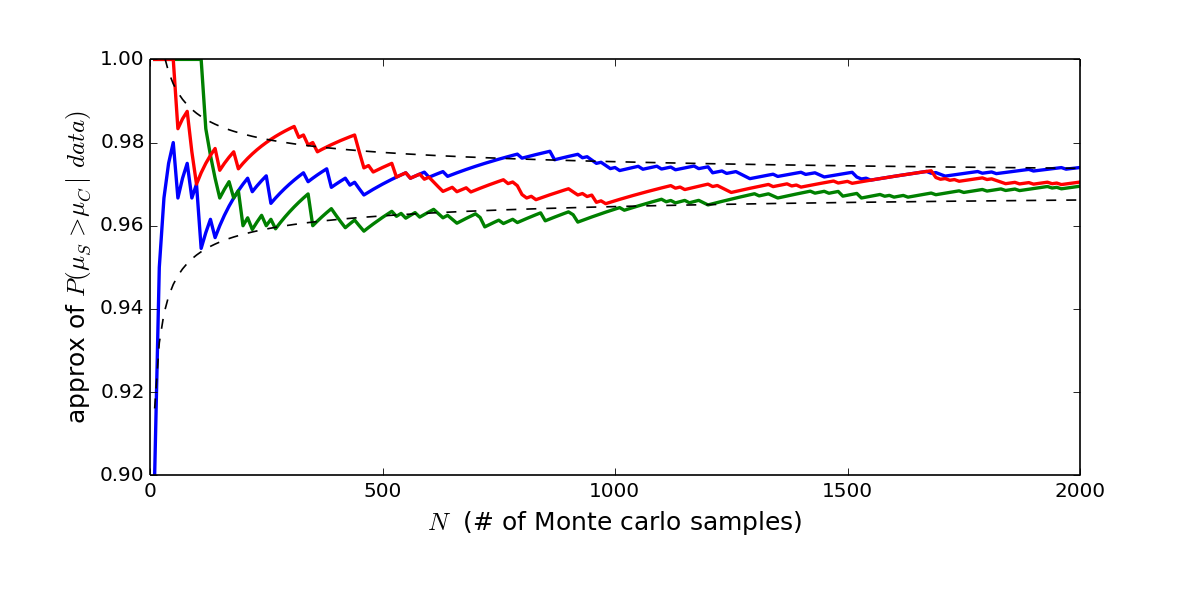
\includegraphics[trim=0 0.75cm 0 0, clip, width=1\textwidth]{pygmalion-MC.png}
    % Source: Original work by J. W. Miller.
  \end{center}
  \caption{Monte Carlo approximations for an increasing number of samples, $N$. The red, blue, and green lines indicate three repetitions of the procedure, using different sequences of samples.  The dotted lines indicate the true value $\pm$ the RMSE of the Monte Carlo estimator.}
  \label{figure:pygmalion-MC}
\end{figure}

In Chapter 4, we saw an example involving the mean change in IQ score $\mu_S$ and $\mu_C$ of two groups of students (spurters and controls). 
To compute the posterior probability that the spurters had a larger mean change in IQ score, we drew $N=10^6$ samples from each posterior:
\begin{align*}
&(\bm\mu_S^{(1)},\bm\lambda_S^{(1)}),\dotsc,(\bm\mu_S^{(N)},\bm\lambda_S^{(N)})\sim \NormalGamma(24.0,8,4,855.0)\\
&(\bm\mu_C^{(1)},\bm\lambda_C^{(1)}),\dotsc,(\bm\mu_C^{(N)},\bm\lambda_C^{(N)})\sim\NormalGamma(11.8,49,24.5,6344.0)
\end{align*}
and used the Monte Carlo approximation
\begin{align*}
\Pr(\bm\mu_S > \bm\mu_C \mid \text{data}) 
\approx \frac{1}{N} \sum_{i = 1}^N \I\big(\bm\mu_S^{(i)}>\bm\mu_C^{(i)}\big).
\end{align*}
To visualize this, consider the sequence of approximations $\frac{1}{N} \sum_{i = 1}^N \I\big(\bm\mu_S^{(i)}>\bm\mu_C^{(i)}\big)$ for $N=1,2,\dotsc$.  Figure \ref{figure:pygmalion-MC} shows this sequence of approximations for three different sets of random samples from the posterior.  We can see that as the number of samples used in the approximation grows, it appears to be converging to around $0.97$.
To visualize the theoretical rate of convergence, the figure also shows bands indicating the true value $\alpha = \Pr(\bm\mu_S > \bm\mu_C \mid \text{data})=0.97$ plus or minus the RMSE of the Monte Carlo estimator, that is, from Equation \ref{equation:RMSE}:
\begin{align*}
\alpha \pm \sigma(X)/\sqrt{N} &= \alpha \pm \sqrt{\alpha(1-\alpha)/N}\\
&= 0.97 \pm \sqrt{0.97(1-0.97)/N}
\end{align*}
where $X$ has the posterior distribution of $\I(\bm\mu_S>\bm\mu_C)$ given the data, in other words, $X$ is a $\Bernoulli(\alpha)$ random variable. 
Recall that the variance of a $\Bernoulli(\alpha)$ random variable is $\alpha(1-\alpha)$.

Using the same approach, we could easily approximate any number of other posterior quantities as well, for example,
\begin{align*}
\Pr\big(\bm\lambda_S>\bm\lambda_C \,\big\vert\, \text{data}\big) 
&\approx \frac{1}{N}\sum_{i = 1}^N \I\big(\bm\lambda_S^{(i)}>\bm\lambda_C^{(i)}\big)\\
\E\big(|\bm\mu_S-\bm\mu_C| \,\big\vert\, \text{data}\big) 
&\approx \frac{1}{N}\sum_{i = 1}^N |\bm\mu_S^{(i)}-\bm\mu_C^{(i)}|\\
\E\big(\bm\mu_S/\bm\mu_C \,\big\vert\, \text{data}\big) 
&\approx \frac{1}{N}\sum_{i = 1}^N \bm\mu_S^{(i)}/\bm\mu_C^{(i)}.
\end{align*}




\subsubsection{Posterior expected loss for resource allocation}
In Chapter 1, we looked at a decision theory example involving allocation of resources for prevention and treatment of a disease. Rather than computing the posterior expected loss using numerical integration, as we did in that example, we could use a Monte Carlo approximation:
\begin{align*}
\rho(c,x) =\E(\ell(\btheta,c)|x) = \int \ell(\theta,c)p(\theta|x)d\theta 
\approx \frac{1}{N}\sum_{i = 1}^N \ell(\btheta_i,c)
\end{align*}
where $\btheta_1,\dotsc,\btheta_N$ are i.i.d.\ samples from the posterior, $p(\theta|x)$.


\subsubsection{Distributions of various posterior quantities}
Posterior samples can also be used to approximate the posterior p.d.f.\ or p.m.f.\ of a complicated quantity, when it might otherwise be difficult to derive. Here's an example.

In the 1998 General Social Survey, respondents were asked about their religious preference and (among other questions) whether they agreed with a Supreme Court ruling prohibiting state and local governments from requiring that certain religious material be read in schools.  Out of the 1011 Protestants in the survey, 353 agreed with the ruling, while out of 860 non-Protestants, 441 agreed.
Suppose that across the entire U.S.\ population, $\theta_p$ and $\theta_n$ are the proportions of Protestants and non-Protestants, respectively, that would agree with the ruling. 

\begin{figure}
  \begin{center}
    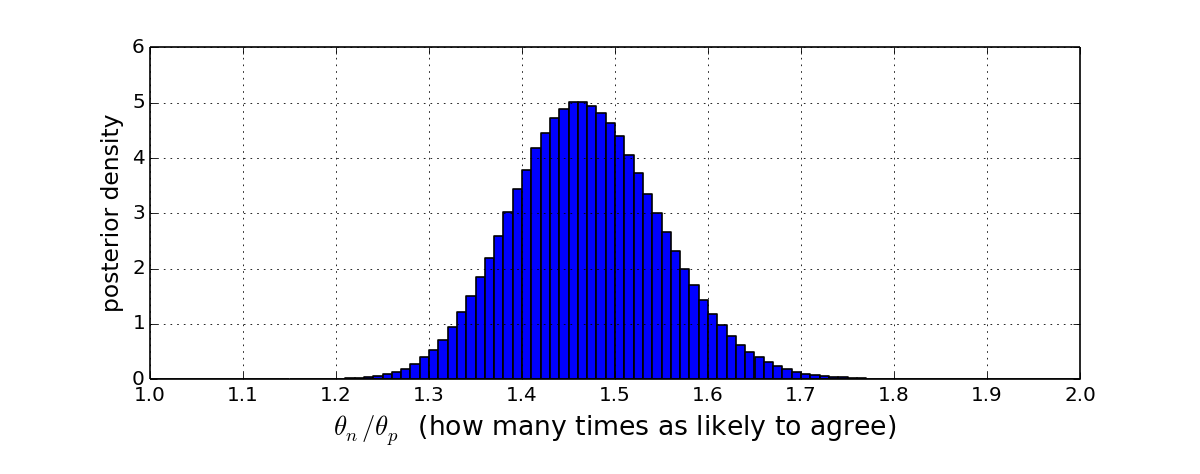
\includegraphics[trim=0 0.65cm 0 0, clip, width=1\textwidth]{Protestant.png}
    % Source: Original work by J. W. Miller.
  \end{center}
  \caption{Estimated posterior density of $\theta_n/\theta_p$ for the Protestant / non-Protestant example.}
  \label{figure:Protestants}
\end{figure}

How many times as likely to agree are non-Protestants than Protestants?
In other words, what is $\theta_n/\theta_p$?
Placing independent uniform priors (that is, $\Beta(1,1)$ priors) on $\theta_p$ and $\theta_n$, and using a binomial model, we find that the posteriors are $\btheta_p|$data $\sim\Beta(354,659)$ and $\btheta_n|$data $\sim\Beta(442,420)$. From this, we can easily construct an approximation to the posterior p.d.f.\ of $\theta_n/\theta_p$ by drawing independent samples 
\begin{align*}
\btheta_p^{(1)},\dotsc,\btheta_p^{(N)}\sim \Beta(354,659)\\
\btheta_n^{(1)},\dotsc,\btheta_n^{(N)}\sim \Beta(442,420)
\end{align*}
and making a histogram (or other density estimate) from the ratios of the samples,
$$\btheta_n^{(1)}/\btheta_p^{(1)},\,\,\dotsc,\,\,\btheta_n^{(N)}/\btheta_p^{(N)}.$$
See Figure \ref{figure:Protestants}.
Note that each bin of the histogram corresponds to a Monte Carlo approximation of the probability of a sample landing in that bin.

% todo: this example is taken from Hoff, p.58.  We could come up with something more recent.

\subsubsection{Approximating the posterior predictive density}

A Monte Carlo approximation to the posterior predictive p.d.f.\ or p.m.f.\ can be made using samples from the posterior:
\begin{align*}
p(x_{n+1}|x_{1:n}) & =\int p(x_{n+1}|\theta) p(\theta|x_{1:n}) d\theta\\
&= \E\big(p(x_{n+1}|\btheta)\mid x_{1:n}\big)\\
&\approx \frac{1}{N}\sum_{i = 1}^N p(x_{n+1}|\btheta_i)
\end{align*}
where $\btheta_1,\dotsc,\btheta_N\iid p(\theta|x_{1:n})$. This is useful when it is difficult or impossible to evaluate the integral analytically.




\section{Importance sampling approximation}
% \section{Importance \xcancel{sampling} approximation}

Importance sampling (IS) is a more powerful type of Monte Carlo approximation. The name ``importance sampling'' is somewhat misleading, since it is not really a method for drawing samples, but rather, a method for approximating expectations---a better name might be importance-weighted approximation. 

\subsubsection*{Advantages of importance sampling over simple Monte Carlo}
\begin{itemize}
\item Can \textit{significantly} improve performance, by reducing the variance
\item Can use samples from a different distribution, say $q$, to compute expectations with respect to $p$
\item Can compute the normalization constant of $p$, as well as Bayes factors
\end{itemize}
\subsubsection*{Disadvantages}
\begin{itemize}
\item Need to be able to evaluate the p.d.f.s/p.m.f.s $p(x)$ and $q(x)$, at least up to proportionality constants
\item It might not be obvious how to choose a good $q$
\end{itemize}

\subsection{The basic idea}
Suppose $X\sim p$ is continuous (the same thing works in the discrete case), and let $q$ be the p.d.f.\ of a distribution we can easily sample from. Assume $q(x)>0$ for all $x$ (or more generally, assume $q(x)>0$ whenever $p(x)>0$; see Section \ref{section:unnormalized}). Then
\begin{align*}
\E h(X) & = \int h(x) p(x) d x \\
& = \int h(x) \frac{p(x)}{q(x)} q(x) d x\\
& \approx \frac{1}{N}\sum_{i = 1}^N h(Y_i) \frac{p(Y_i)}{q(Y_i)}
\end{align*}
where $Y_1,\dotsc,Y_N\iid q$, is called an \term{importance sampling approximation}. The approximation step here is just a simple Monte Carlo approximation, as in Section \ref{section:Monte-Carlo}. The distribution $q$ is sometimes called the \term{proposal distribution}. The ratios $w(Y_i) = p(Y_i)/q(Y_i)$ are referred to as the \term{importance weights}. The intuitive interpretation is that the importance weights correct for the fact that we are sampling from $q$ rather than $p$, since $y$'s that occur less frequently under $q$ than $p$ have large importance weight $w(y)$ (and $y$'s that occur more frequently under $q$ then $p$ have small importance weight).  

For the basic IS approximation described above, it is necessary to be able to evaluate $p(x)$ and $q(x)$ in order to compute the importance weights.  There is a more general version for which $p(x)$ and $q(x)$ only need to be computable up to constants of proportionality; see Section \ref{section:unnormalized}.

\subsubsection{Basic properties}
Since this is essentially just a Monte Carlo approximation, it has all the properties described in Section \ref{section:Monte-Carlo}: 
\begin{itemize}
\item consistent, as long as $\E|h(Y) p(Y)/q(Y)|<\infty$, where $Y \sim q$
\item unbiased
\item the variance of the estimator is $\frac{1}{N}\V\big(h(Y) p(Y)/q(Y)\big)$
\item the RMSE is $\sigma\big(h(Y)p(Y)/q(Y)\big)/{\sqrt N}$.
\end{itemize}
So, the rate of convergence is still of order $1/\sqrt N$, however, the constant $\sigma\big(h(Y)p(Y)/q(Y)\big)$ may be smaller or larger than the constant $\sigma\big(h(X)\big)$ of the more direct estimator $\frac{1}{N}\sum h(X_i)$.

\subsubsection{Choosing the proposal distribution}
\label{section:choosing-q}
To minimize the RMSE, we want $q(x)$ to look as much like $h(x)p(x)$ as possible, up to a constant of proportionality. In fact, if we could choose $q(x)$ to be exactly proportional to $h(x)p(x)$, then we would have $h(x)p(x)/q(x)=c$ for some $c$, and this would mean that $\sigma\big(h(Y)p(Y)/q(Y)\big)=0$, in other words, the error would be zero after only one sample!  In this situation, however, there would be no need to resort to sampling at all, since in this case, $\E h(X) = h(x)p(x)/q(x)$ for any $x$, so if we can compute $h(x)p(x)/q(x)$ then we already know $\E h(X)$.

Nonetheless, this indicates that to minimize the approximation error, we want $q(x)$ to be as close as possible to being proportional to $h(x) p(x)$, and it shows that there can be a substantial reduction in the error if a good choice of $q(x)$ is made. When choosing $q$, it is usually better to err on the side of having it a little more ``spread out'', to make sure that it sufficiently covers the area where $h(x) p(x)$ is large, rather than not covering some of this area (because that would result in occasionally having very large importance weights, which would increase the RMSE of the estimator).

That said, in practice, we often want to estimate $\E h(X)$ for a variety of different functions $h$. Because of this, a common practice is to choose $q(x)$ to be as close as possible to $p(x)$ (rather than $h(x) p(x)$), so that we can reuse the same samples and the same importance weights, and still obtain reasonably good estimators for all of these $h$'s, rather than specializing for each individual $h$.

\subsection{Example: Marginal likelihood under a non-conjugate prior}
\label{section:gps}

\begin{figure}
  \begin{center}
    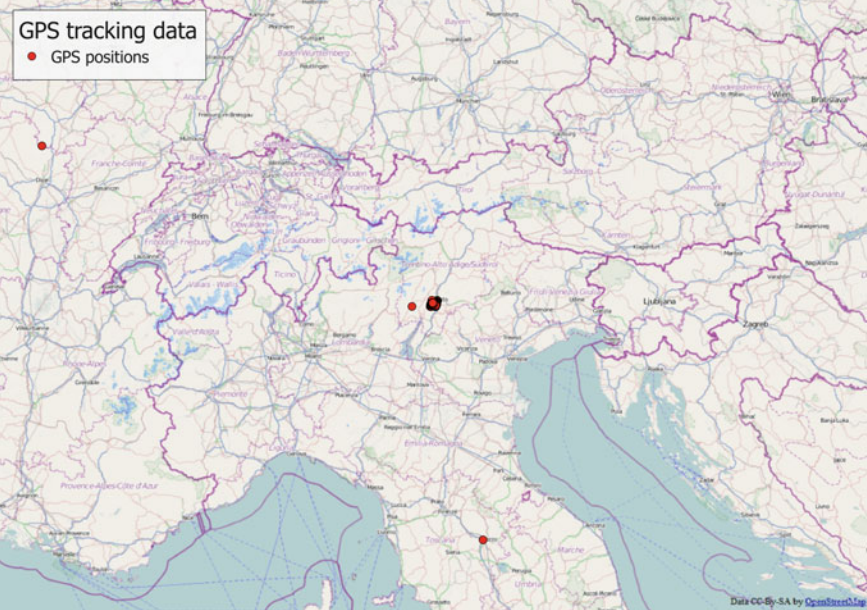
\includegraphics[width=0.8\textwidth]{urbano-GPS-outliers.png}
    % Source: http://ase-research.org/basille/pubs/Urbano_2014b.pdf
    %   Urbano, Ferdinando, Mathieu Basille, and Francesca Cagnacci. "Data Quality: Detection and Management of Outliers." Spatial Database for GPS Wildlife Tracking Data. Springer International Publishing, 2014. 115-137.
    % License: ???
    % Date accessed: 1/31/2014
  \end{center}
  \caption{Animal-tracking GPS measurements, with extreme outliers. (Urbano et al., 2014)}
  \label{figure:urbano-GPS-outliers}
\end{figure}

In wildlife management and conservation, animals are tagged with GPS devices in order to track their movements and study their behavior. The latitude/longitude measurements made by GPS devices are usually fairly accurate, but it is not uncommon to get extreme outliers. For instance, Figure \ref{figure:urbano-GPS-outliers} (Urbano et al., 2014) shows GPS measurements in northern Italy, with three extreme outliers visible---one of which is way down toward central Italy, and another of which is clear across Switzerland and well into France!  The Normal (Gaussian) model is not robust to outliers, and if used naively in a situation like this, would give completely bogus results.

One approach to dealing with outliers is to identify and remove them, but this can be somewhat subjective, and can be difficult in high-dimensional settings where the data cannot easily be visualized. Another approach is to use a heavy-tailed distribution instead of the Normal, such as the Laplace distribution, Cauchy distribution, or $t$-distribution. A difficulty that arises, however, is that these distributions do not have nice conjugate priors, so we cannot do inference analytically. One way to do inference in such a situation is using importance sampling.

To illustrate, consider the following 8 latitude/longitude points, one of which is an outlier:

\begin{center}
\begin{tabular}{ll}
Latitude & Longitude \\
\hline
36.077916 N & 79.009266 W \\
36.078032 N & 79.009180 W \\
36.078129 N & 79.009094 W \\
36.078048 N & 79.008891 W \\
36.077942 N & 79.008962 W \\
36.089612 N & 79.035760 W \\
36.077789 N & 79.008917 W \\
36.077563 N & 79.009281 W \\
\end{tabular}
\end{center}

To keep things simple, let's just consider the latitudes, and let's assume these points are collected in a short enough amount of time that the animal has not moved very far. See the histogram of the latitudes in Figure \ref{figure:gps-histogram}. Let's model the latitudes as
$$X_1,\ldots,X_n\iid \Cauchy(\theta,s).$$
Recall that the Cauchy distribution with location $\theta$ and scale $s$ has p.d.f.
$$\Cauchy(x\mid \theta, s) = \frac{1}{\pi s \Big(1 + \big(\frac{x-\theta}{s}\big)^2\Big)}.$$
Unfortunately, there is not a nice conjugate prior for $\theta$. Let's put a Cauchy prior on $\theta$:
$$\btheta\sim \Cauchy(\theta_0,s_0).$$

\subsubsection*{Parameter settings}
\begin{itemize}
    \item scale of measurement errors: $s = 0.0002$ degrees (known, say, from calibration testing or instrument specifications)
    \item center of prior on location: $\theta_0 = 36.07$ degrees (estimated, say, from many previous measurements for this animal)
    \item scale of prior on location: $s_0 = 0.02$ degrees (estimated, say, from many previous measurements for this animal)
\end{itemize}



\begin{figure}
  \begin{center}
    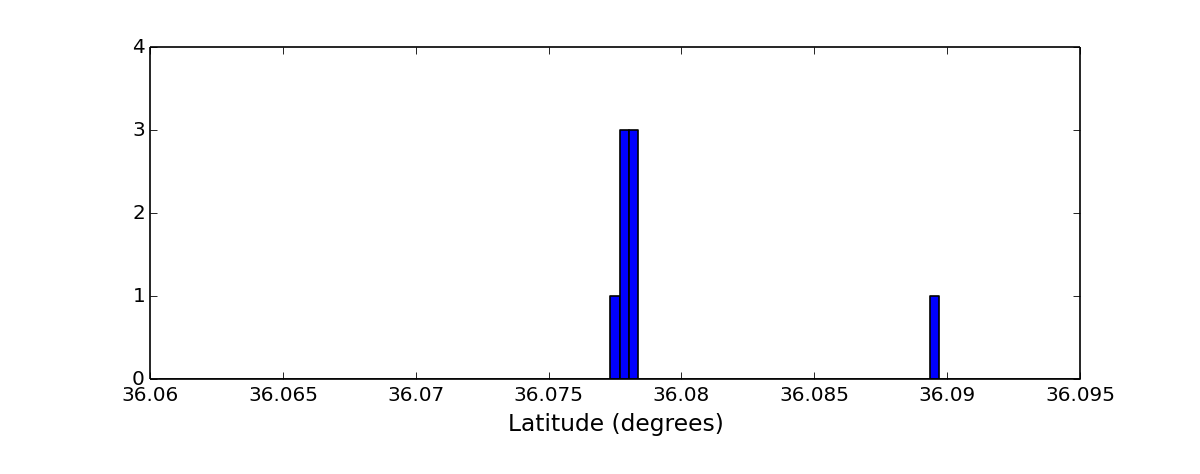
\includegraphics[trim=0 0.75cm 0 0, clip, width=1\textwidth]{gps-histogram.png}
    % Source: Original work by Jeffrey W. Miller
    % Date: 1/31/2014
  \end{center}
  \caption{Histogram of latitude measurements.}
  \label{figure:gps-histogram}
\end{figure}

\begin{figure}
  \begin{center}
    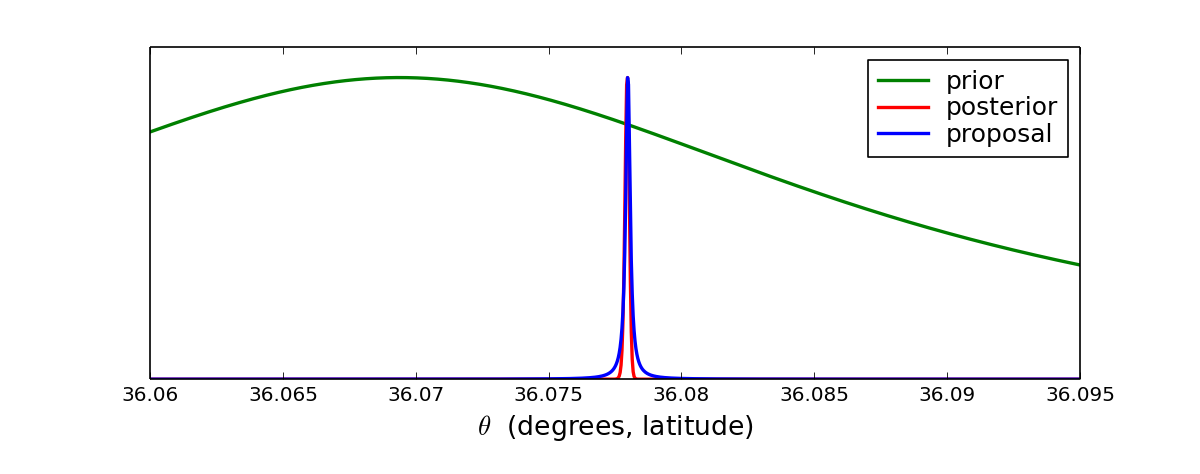
\includegraphics[trim=0 0.65cm 0 0, clip, width=1\textwidth]{gps-curves.png}
    % Source: Original work by Jeffrey W. Miller
    % Date: 1/31/2014
  \end{center}
  \caption{Prior, posterior, and proposal densities. (NOTE: To make them all visible on the same plot, each curve is scaled so that the maximum is 1.)}
  \label{figure:gps-curves}
\end{figure}

\begin{figure}
  \begin{center}
    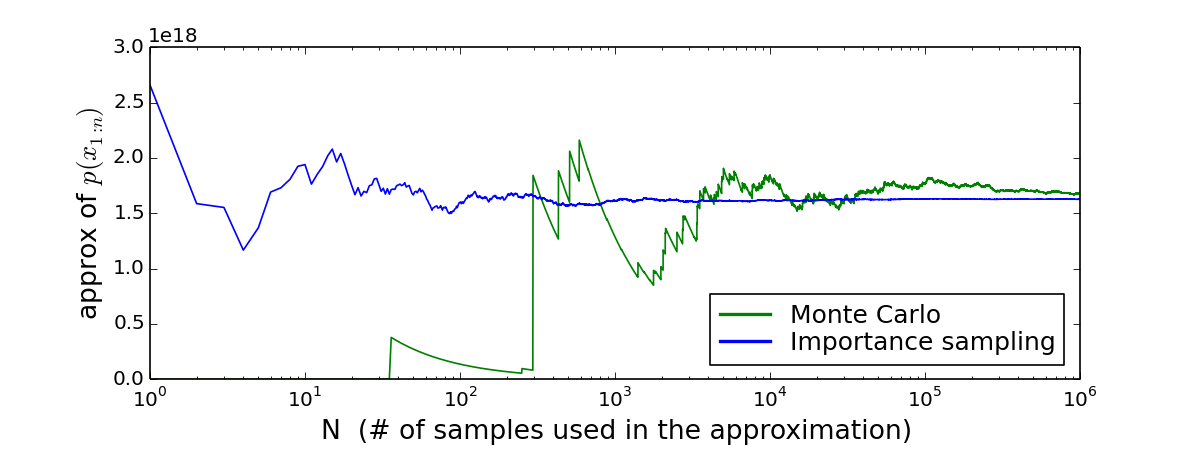
\includegraphics[trim=0 0.65cm 0 0, clip, width=1\textwidth]{gps-convergence.png}
    % Source: Original work by Jeffrey W. Miller
    % Date: 1/31/2014
  \end{center}
  \caption{Sequence of approximations for $N = 1,\dotsc,10^6$, for Monte Carlo and importance sampling. Nota bene: The x-axis is on the log scale.}
  \label{figure:gps-convergence}
\end{figure}

\subsubsection*{Approximating the marginal likelihood}
Suppose we need to know the marginal likelihood $p(x_{1:n})$. (This is needed, for example, when doing inference over multiple models, as we will see later.) Since we can't compute it analytically (as far as I know), an approximation is needed. One approach would be a simple Monte Carlo approximation:
\begin{align}\label{equation:gps-MC}
p(x_{1:n}) =\int p(x_{1:n}|\theta) p(\theta) d\theta
\approx\frac{1}{N}\sum_{i = 1}^N p(x_{1:n}|\btheta_i)
% & =\frac{1}{N}\sum_{i = 1}^N \Big(\prod_{j = 1}^n p(x_j|\btheta_i)\Big).
\end{align}
where $\btheta_1,\dotsc,\btheta_N\iid p(\theta)$ (i.i.d.\ from the prior). Although this works asymptotically, it is a very poor approximation (the RMSE is large). We can do much better with importance sampling, for a good choice of $q$:
\begin{align}\label{equation:gps-IS}
p(x_{1:n}) = \int p(x_{1:n}|\theta) \frac{p(\theta)}{q(\theta)}q(\theta) d\theta 
 \approx\frac{1}{N}\sum_{i = 1}^N p(x_{1:n}|\btheta_i) \frac{p(\btheta_i)}{q(\btheta_i)}
\end{align}
where $\btheta_1,\dotsc,\btheta_N\iid q(\theta)$ (i.i.d.\ from $q$). As discussed in Section \ref{section:choosing-q}, we want $q(\theta)$ to look as
much like $p(x_{1:n}|\theta) p(\theta)$ as possible, and if necessary, to err on the side of being a little more spread out. By cheating (a little bit) and looking at a plot of the posterior, let's choose
$$q(\theta) = \Cauchy(\theta\mid \median(x_{1:n}), 10^{-4}).$$
(A more principled choice could be made based on the rate of convergence of the posterior, but that would be more involved.)  See Figure \ref{figure:gps-curves} for plots of the prior, posterior, and proposal distribution $q$.

\subsubsection*{Results}
To visualize the rate of convergence, Figure \ref{figure:gps-convergence} shows a sequence of Monte Carlo approximations (Equation \ref{equation:gps-MC}) and importance sampling approximations (Equation \ref{equation:gps-IS}) for $N=1,\ldots,10^6$.
The IS approximations appear to converge much more quickly, by several orders of magnitude.

Why does this happen? From Figure \ref{figure:gps-curves} we can see that the prior is so spread out, compared to the posterior (and thus, the likelihood), that samples from the prior very rarely land in the small region where the likelihood is large.  So most of the terms in the Monte Carlo approximation are essentially zero, and a small number of them are enormous (making the variance, and thus the RMSE, large). This situation is typical when approximating the marginal likelihood, since the posterior becomes more and more concentrated as the size of the dataset grows. (In fact, typically the situation is much worse---here, $n$ is only eight!)

A general word of caution: Approximating the marginal likelihood can be a tricky business, and one needs to be careful when going about it.

% The likelihood is
% \begin{align*}
% p(x_{1:n}) = \prod_{i = 1}^n \Cauchy(x_i\mid\theta,s)
 % = \prod_{i = 1}^n \frac{1}{\pi s \Big(1 + \big(\frac{x_i-\theta}{s}\big)^2\Big)}.
% \end{align*}

% \begin{align*}
% p(\theta|x_{1:n})&\propto \Cauchy(\theta\mid\theta_0,s_0)\prod_{i = 1}^n \Cauchy(x_i\mid\theta,s)\\
% & = \frac{1}{\pi s_0 \Big(1 + \big(\frac{\theta-\theta_0}{s_0}\big)^2\Big)}
    % \prod_{i = 1}^n \frac{1}{\pi s \Big(1 + \big(\frac{x_i-\theta}{s}\big)^2\Big)}.
% \end{align*}



%Here's one way of thinking about importance sampling: Suppose we want to approximate $\E h(X)$ where $X\sim p$, but we can't sample from $p$ because it is too complicated. However, suppose we can easily sample from $q$, which is very similar to $p$. Is there some way we can use samples from $q$, and correct for the discrepancy between $p$ and $q$, to still get an asymptotically correct approximation of $\E h(X)$? The answer is yes (of course), and here's how. 


\subsection{Handling unknown normalization constants}
\label{section:unnormalized}
As described so far, in order to implement an importance sampling approximation, it looks like we need to be able to compute the p.d.f./p.m.f.\ values $p(Y_i)$ and $q(Y_i)$. In many cases, it is not possible to compute $p$ and $q$ themselves, but often, we will be able to compute functions $\tilde p$ and $\tilde q$ proportional to $p$ and $q$. Fortunately, there is a neat little trick that still allows us to make an IS approximation. Suppose
\begin{align*}
p(x) &= \tilde p(x)/Z_p\\
q(x) &= \tilde q(x)/Z_q
\end{align*}
where $\tilde p(x)$ and $\tilde q(x)$ are easy to compute (but $Z_p$ and $Z_q$ may be intractable). Also, rather than assuming $q(x)>0$ for all $x$, let us assume only that $\tilde q(x)>0$ whenever $\tilde p(x)>0$. Define
$$\tilde w(x) = \branch{\tilde p(x)/\tilde q(x)}{\tilde q(x)>0}{0}{\tilde q(x)=0.}$$
The general form of an importance sampling approximation is then
\begin{align}\label{equation:general-IS}
\E h(X) = \int h(x)p(x)d x \approx\frac{\frac{1}{N}\sum_{i = 1}^N h(Y_i) \tilde w(Y_i)}{\frac{1}{N}\sum_{i = 1}^N \tilde w(Y_i)}
= \sum_{i = 1}^N h(Y_i) \left(\frac{\tilde w(Y_i)}{\sum_{j = 1}^N \tilde w(Y_j)}\right)
\end{align}
where $Y_1,\dotsc,Y_N\iid q$. (See derivation in Section \ref{section:IS-derivation}). This can be interpreted as a weighted average of the $h(Y_i)$'s, with weights $\tilde w(Y_i)/\sum_j \tilde w(Y_j)$. 


\subsubsection{Example: Approximating posterior expectations}
Consider the animal-tracking GPS example from Section \ref{section:gps}, and now suppose we would like to estimate the posterior mean. Define
\begin{align*}
    & \pi(\theta) = p(\theta|x_{1:n})\\
    & \tilde \pi(\theta) = p(x_{1:n}|\theta)p(\theta)\\
    & Z_\pi = p(x_{1:n}) = \int p(x_{1:n}|\theta)p(\theta)d\theta = \int \tilde\pi(\theta)d\theta.
\end{align*}
Then $\pi(\theta) = \tilde \pi(\theta) / Z_\pi$, and using Equation \ref{equation:general-IS},
\begin{align*}
    \E(\btheta|x_{1:n}) = \int \theta p(\theta|x_{1:n})d\theta = \int \theta \pi(\theta)d\theta
    \approx \frac{\frac{1}{N}\sum_{i = 1}^N \btheta_i \tilde w(\btheta_i)}{\frac{1}{N}\sum_{i = 1}^N \tilde w(\btheta_i)}
\end{align*}
where $\btheta_1,\ldots,\btheta_N\iid q$ and $\tilde w(\theta) = \tilde \pi(\theta) / q(\theta)$.  For the data from Section \ref{section:gps}, with $N=10^6$, this yields an approximate value of $\E(\btheta|x_{1:n}) \approx 36.0780$. Note that, in this example, since $Z_q$ is effectively 1, the denominator in this approximation is identical to the IS approximation of $Z_\pi$ that we used in Section \ref{section:gps}.  More generally, however, the denominator will be an approximation of the ratio of normalization constants (see Section \ref{section:IS-derivation}).



\subsubsection{Derivation of Equation \ref{equation:general-IS}}
\label{section:IS-derivation}
Letting $S = \{x:\tilde p(x)>0\}$, we have
\begin{align*}
\E h(X) & =  \int h(x) p(x) d x \\
& = \int_S h(x) \frac{\tilde p(x)}{Z_p} d x \\
& \overset{\text{(a)}}{=} \int_S h(x) \frac{\tilde p(x)}{Z_p}\frac{Z_q}{\tilde q(x)} q(x) d x \\
& = \frac{Z_q}{Z_p} \int_S h(x) \tilde w(x) q(x) d x\\
& \overset{\text{(b)}}{=} \frac{Z_q}{Z_p} \int h(x) \tilde w(x) q(x) d x\\
& \overset{\text{(c)}}{\approx} \frac{Z_q}{Z_p} \frac{1}{N}\sum_{i = 1}^N h(Y_i) \tilde w(Y_i)
\end{align*}
where in step (a), we use the assumption that $\tilde q(x)>0$ whenever $\tilde p(x)>0$, in step (b), we use the fact that $\tilde w(x)=0$ for any $x\not\in S$, and step (c) is a simple Monte Carlo approximation.  Similarly, for the ratio of normalizing constants $Z_p/Z_q$,
\begin{align*}
\frac{Z_p}{Z_q} & = \frac{1}{Z_q}\int \tilde p(x) d x\\
& = \frac{1}{Z_q}\int_S \tilde p(x) d x\\
& = \frac{1}{Z_q}\int_S \frac{\tilde p(x)}{\tilde q(x)}\tilde q(x) d x\\
& = \int_S \frac{\tilde p(x)}{\tilde q(x)}q(x) d x\\
& = \int \tilde w(x)q(x) d x\\
& \approx \frac{1}{N}\sum_{i = 1}^N \tilde w(Y_i).
\end{align*}







\section{Basic techniques for generating samples}

\subsection{Inverse c.d.f.\ method / Smirnov transform}

The \term{inverse c.d.f.\ method} or \term{Smirnov transform} is a common way of generating random samples from
univariate probability distributions when the inverse of the c.d.f.\ can be easily computed.
The basic idea is that if $U\sim\Uniform(0,1)$ and $G$ is the inverse (in a generalized sense) of the c.d.f.\ $F$, then $G(U)$ is a random variable with c.d.f.\ $F$.

\subsubsection{Example: Sampling from $\Exp(\theta)$}
The $\Exp(\theta)$ c.d.f.\ is $F(x) = (1-e^{-\theta x})\I(x>0)$. This is invertible on $(0,\infty)$, with inverse $G(u)=-(1/\theta)\log(1-u)$ for $u\in(0,1)$. Therefore, if $U\sim\Uniform(0,1)$ then $G(U)\sim \Exp(\theta)$.

\subsubsection{A precise statement of the method}

\begin{proposition}\label{proposition:inverse}
    Let $F$ be a c.d.f.\ on $\R$, and define $G(u) =\inf \{x\in\R: F(x)\geq u\}$ for $u\in(0,1)$. If $U\sim\Uniform(0,1)$, then $G(U)\sim F$.
\end{proposition}
See Appendix for proof.

\subsubsection*{Remarks}
\begin{itemize}
\item If $F$ is invertible, then $G = F^{-1}$.  The definition of $G$ above is a generalized inverse that allows for the possibility that $F$ has discontinuities and/or is constant on certain intervals.
\item $G(u)\in\R$ for any $u\in(0,1)$ since $F(x)\to 1$ as $x\to\infty$, and $F(x)\to 0$ as $x\to-\infty$.
\item By convention, $F$ is assumed to be continuous from the right, rather than the left.
\end{itemize}



% \subsubsection{A precise statement of the method (Version 2)}
% Let $F$ be a c.d.f.\ on $\R$, and define $F(-\infty) = 0$, $F(\infty) = 1$. Let $G$ be monotone increasing on $(0,1)$, and define $G(0) =-\infty$, $G(1) =\infty$. Suppose $G$ is a generalized inverse of $F$ in the sense that
% \begin{itemize}
% \item for any $x\in\R$, $G(F(x))\leq x$, and
% \item for any $u\in(0,1)$, $u\leq F(G(u))$.
% \end{itemize}
% If $U\sim\Uniform(0,1)$ then $G(U)\sim F$.
% \subsubsection*{Proof}
% Let $u\in(0,1)$ and $x\in\R$. If $u\leq F(x)$ then $G(u)\leq G(F(x))\leq x$. If $G(u)\leq x$ then $u\leq F(G(u))\leq F(x)$. Hence, for any $u\in(0,1)$, $x\in\R$, we have $u\leq F(x)$ if and only if $G(u)\leq x$. Let $U\sim\Uniform(0,1)$. Then for any $x\in\R$,
% $$\Pr(G(U)\leq x) =\Pr(U\leq F(x)) = F(x). $$
% Hence, $G(U)$ has c.d.f.\ $F$.




\subsection{Rejection sampling}

Rejection sampling is a method for drawing random samples from a distribution whose p.d.f.\ can be evaluated up to a constant of proportionality. Compared with the inverse c.d.f.\ method, rejection sampling has the advantage of working on complicated multivariate distributions, however, one has to design a good proposal distribution (which can be difficult, especially in high-dimensional settings).
%Compared with importance sampling, rejection sampling has the advantage of generating samples exactly from the desired distribution, however, it is typically less efficient than importance sampling for approximating expectations.

The method relies on two principles:
\begin{enumerate}
\item \textbf{The rejection principle:} Rejecting results in conditional samples. That is, if we reject any samples falling outside of a given set, the remaining samples are distributed according to the conditional distribution on that set.
\item \textbf{The projection principle:} A distribution equals the projection of the uniform distribution under its p.d.f.  That is, if we sample uniformly from the region under the p.d.f.\ (or a function proportional to it) of a distribution, and discard the ``height'', we obtain a sample from that distribution.
\end{enumerate}

\subsubsection{The rejection principle} 

\begin{figure}
  \begin{center}
    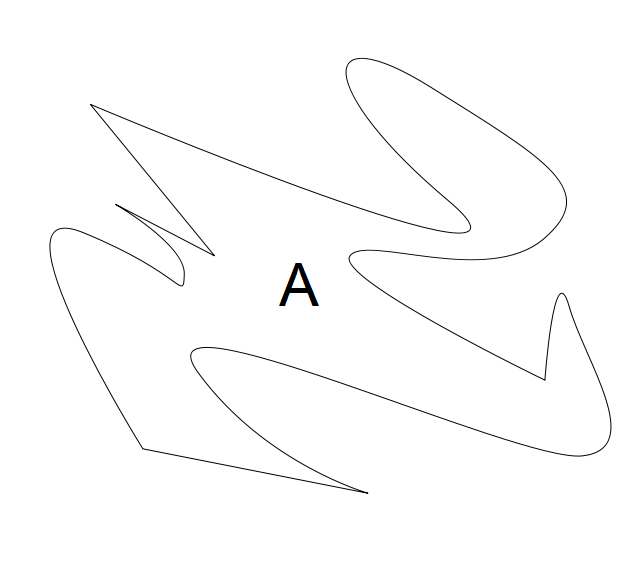
\includegraphics[width=0.45\textwidth]{reject-wo-samples.png}
    \hspace{0.05\textwidth}
    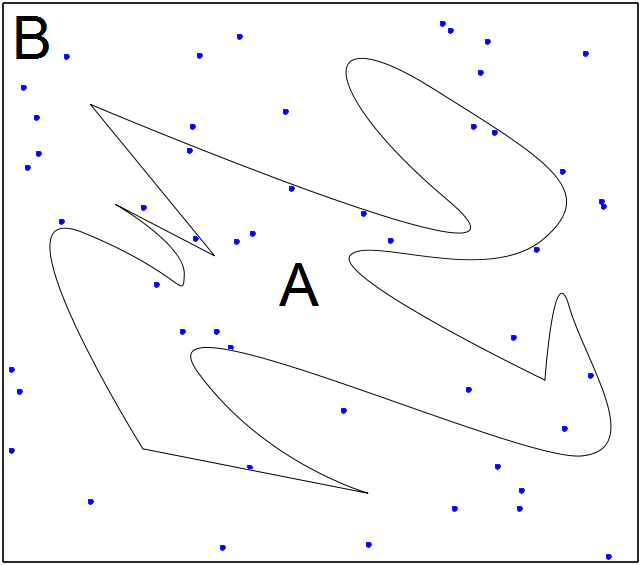
\includegraphics[width=0.45\textwidth]{reject-w-samples.png}
    % Source: Original work by Jeffrey W. Miller
    % Date: 2/1/2014
  \end{center}
  \caption{(Left) How to draw uniform samples from region $A$? (Right) Draw uniform samples from $B$ and keep only those that are in $A$.}
  \label{figure:reject}
\end{figure}

Consider the oddly-shaped two-dimensional region $A$ in Figure \ref{figure:reject}. How would you generate samples uniformly over $A$? In other words, how would you generate samples from $\Uniform(A)$, the uniform distribution on $A$? The rejection sampling approach is to choose a simpler region $B$ containing $A$, generate samples from $\Uniform(B)$, and keep only the samples that land inside $A$. The name ``rejection sampling'' comes from the fact that we discard, or ``reject'', any samples landing outside $A$.
It turns out that this is guaranteed to generate samples from $\Uniform(A)$.
In fact, more generally, rejecting results in samples from the conditional distribution on $A$; see Proposition \ref{proposition:reject}.

In order to be as efficient as possible, we want the bounding region $B$ to be as small as possible (while still containing $A$), so that the number of rejections is kept to a minimum.


\subsubsection{The projection principle}

Suppose we want to sample from a distribution on $\R^d$ with p.d.f.\ $\pi(x)=\tilde \pi(x)/Z_\pi$. Consider the region of $\R^{d+1}$ under $\tilde \pi$:
$$ A =\Big\{(x,y): x\in\R^d,\,0<y<\tilde \pi(x)\Big\}. $$
It turns out that if $(X,Y)\sim\Uniform(A)$ (that is, $(X,Y)$ is uniformly distributed over $A$), then $X\sim \pi$.

To see why, first note that the volume of $A$ is
$$\Vol(A) = \int \tilde \pi(x) d x = \int Z_\pi \pi(x) d x = Z_\pi, $$
and since the p.d.f.\ of the uniform distribution on $A$ is constant, we have
$$p(x,y) = \Uniform(x,y\mid A) = \frac{\I\big((x,y)\in A\big)}{\Vol(A)} = \frac{\I\big(0<y<\tilde \pi(x)\big)}{Z_\pi}.$$
Therefore,
\begin{align*}
p(x) & =\int_{-\infty}^\infty p(x,y) d y = \int_{-\infty}^\infty \frac{\I\big(0<y<\tilde \pi(x)\big)}{Z_\pi} d y\\
& = \frac{1}{Z_\pi} \int_0^{\tilde \pi(x)} d y = \frac{\tilde \pi(x)}{Z_\pi} = \pi(x).
\end{align*}


\subsubsection{The rejection sampling procedure}
Combining these two principles leads to the following procedure. Suppose we want to draw samples from a distribution on $\R^d$ with p.d.f.\ $p(x) \propto \tilde p(x)$.
\begin{itemize}
\item Choose a proposal distribution $q$ that is easy to sample from, and is as close as possible to being proportional to $\tilde p$.
\item Choose $c>0$ such that $ c q(x)\geq \tilde p(x)$ for all $x$.
\end{itemize}
To draw a sample from $p$:
\begin{enumerate}
\item Sample $X\sim q$.
\item Sample $Y\sim\Uniform(0,c q(X))$.
\item If $Y \geq \tilde p(X)$, then go back to step 1.
\item Otherwise, output $X$ as a sample.
\end{enumerate}
Then the accepted $X$'s are distributed according to $p$. To see why, let
\begin{align*}
A &= \Big\{(x,y): x\in\R^d,\,0<y<\tilde p(x)\Big\}\\
B &= \Big\{(x,y): x\in\R^d,\,0<y<c q(x)\Big\}
\end{align*}
and note that
\begin{itemize}
\item steps 1 and 2 generate a sample $(X,Y)$ uniformly from $B$, since their joint density is
    $$q(x)\Uniform\big(y\mid (0,\,c q(x))\big) = q(x) \frac{\I\big(0<y<c q(x)\big)}{c q(x)} = \frac{\I\big((x,y)\in B\big)}{c},$$
\item step 3 rejects any pairs $(X,Y)$ that are outside of $A$, so that the distribution of accepted pairs is uniform on $A$ (by the rejection principle), and
\item step 4 keeps only $X$, resulting in a sample from $p$ (by the projection principle).
\end{itemize}


% todo: future: example


% \section{Variance-reduction techniques}
% future?


% \section{History}

% Fermi story
% Ulam, picture with physical simulator, from Stan manual?

%\newpage
\section{Exercises}

\begin{enumerate}
\item The Gumbel distribution with location $c\in\R$ and scale $\beta>0$ has c.d.f.\
$$ F(x\mid c,\beta) = \exp\big(-e^{-(x-c)/\beta}\big) .$$
This distribution has certain special properties that make it well-suited for modeling extreme values, and it is often used in hydrology as a model for measurements such as the maximum annual water level of a river, or maximum monthly rainfall in a region. Use the inverse c.d.f.\ method to derive a procedure for generating $\Gumbel(c,\beta)$ random variables from $\Uniform(0,1)$ random variables.
\item When $X\sim\Cauchy(0,1)$, we have $\E|X|=\infty$, and thus the Monte Carlo approximations $\frac{1}{N}\sum_{i = 1}^N X_i$ are not guaranteed to converge as $N\to\infty$, when $X_1,X_2,\dotsc\iid \Cauchy(0,1)$ (indeed, the mean $\E X$ does not even exist for the Cauchy distribution).  Explore what happens empirically by sampling $X_1,\dotsc,X_M\iid \Cauchy(0,1)$ for $M=10^6$ and plotting the sequence of Monte Carlo approximations for $N = 1,\dotsc,M$. Do this for several sets of samples $X_1,\dotsc,X_M$, and pick four representative examples to display in separate plots. Discuss what you see.
\item The ``harmonic mean approximation'' of the marginal likelihood is
$$ p(x_{1:n}) \approx \frac{1}{\frac{1}{N}\sum_{i = 1}^N 1/p(x_{1:n}|\btheta_i)}$$
where $\btheta_1,\dotsc,\btheta_N\iid p(\theta|x_{1:n})$ (that is, they are i.i.d.\ from the posterior).
\begin{enumerate}
\item Show that, in principle, this converges to the marginal likelihood $p(x_{1:n})$. Assume that $p(x_{1:n}|\theta)>0$ for all $\theta$.
\item Consider the following simple example with $n=1$: $X_1\sim \N(\theta,\lambda^{-1})$ with $\lambda=1$, and
    $\btheta\sim\N(0,\lambda_0^{-1})$ with $\lambda_0=1/10^2$.
    Compute the harmonic mean approximation for $p(x_1)$ when $x_1=2$, using $N=10^6$.
    Report the result for 5 independent sets of samples $\btheta_1,\ldots,\btheta_N$ from the posterior.  
    Compare these with the true value of the marginal likelihood, $\N(2\mid 0,\lambda^{-1}+\lambda_0^{-1})$.  Describe what you observe.
    (This example is due to Neal, 2008).
\item Repeat part (b) using $\lambda_0 = 1/100^2$.
\end{enumerate}
The harmonic mean approximation was fairly popular for a while, since it is so easy to compute from posterior samples (which we will often have from running MCMC, stay tuned), however, it can have extremely poor performance. Importance sampling, and related methods such as path sampling, are far better.
\item Implement both the Monte Carlo and importance sampling approximations to the marginal likelihood for the GPS example in Section \ref{section:gps}. Create a plot like Figure \ref{figure:gps-convergence}, to visualize the convergence of the approximations.
\item Suppose $A\subset\R^d$ and $X,X_1,X_2,\dotsc\in\R^d$ are i.i.d. with $\Pr(X\in A)>0$. Show that if $Z = X_K$ where $K =\min\{k: X_k\in A\}$, then $Z \overset{D}{=} (X\mid X\in A)$, that is, $Z$ has the same distribution as $X\mid X\in A$. Do this by showing that $\Pr(Z\in S) = \Pr(X\in S\mid X\in A)$ for any $S\subset A$. (Hint: $\sum_{k = 0}^\infty a^k = 1/(1-a)$ for $a\in[0,1)$.)
\end{enumerate}

% future: Newcomb outlier detection






\section*{Supplementary material}
\begin{itemize}
\item Hoff (2009), 4.1 and 4.2.
\item mathematicalmonk videos, Machine Learning (ML) 17.1--17.14 \\ 
    \url{https://www.youtube.com/playlist?list=PLD0F06AA0D2E8FFBA}
\end{itemize}

\section*{References}
\begin{itemize}
\item Urbano, F., Basille, M., and Cagnacci, F. Data Quality: Detection and Management of Outliers. Spatial Database for GPS Wildlife Tracking Data. Springer International Publishing, 2014. 115-137.
\item Radford Neal (2008), The Harmonic Mean of the Likelihood: Worst Monte Carlo Method Ever. 
\url{https://radfordneal.wordpress.com/2008/08/17/the-harmonic-mean-of-the-likelihood-worst-monte-carlo-method-ever/}
\end{itemize}



\appendix
\section*{Proofs}

\begin{proof}[Proof of Proposition \ref{proposition:inverse}]
First, we show that for any $u\in(0,1)$, $x\in\R$, we have 
\begin{align}\label{equation:iff}
u\leq F(x) \text{ if and only if } G(u)\leq x.
\end{align}
If $u\leq F(x)$ then
$$ G(u) =\inf\{y\in\R: u\leq F(y)\}\leq x $$
because $x\in\{y\in\R: u\leq F(y)\}$. On the other hand, suppose $G(u)\leq x$. Then there exist $x_1\geq x_2\geq \cdots$ such that $x_n\to G(u)$ and $u\leq F(x_n)$ for all $n$. Thus,
$$ u\leq\liminf F(x_n) \overset{\text{(a)}}{=} F(G(u))\overset{\text{(b)}}{\leq} F(x) $$
where (a) is because $F$ is continuous from the right, and (b) is because $F$ is monotone increasing. This proves Equation \ref{equation:iff}.

Therefore, for any $x\in\R$,
$$\Pr(G(U)\leq x) =\Pr(U\leq F(x)) = F(x). $$
Hence, $G(U)$ has c.d.f.\ $F$.
\end{proof}


\begin{proposition}\label{proposition:reject}
Suppose $A\subset\R^d$ and $X,X_1,X_2,\dotsc\in\R^d$ are i.i.d. with $\Pr(X\in A)>0$. If $Z = X_K$ where $K =\min\{k: X_k\in A\}$, then $Z \overset{D}{=} (X\mid X\in A)$, that is, $Z$ has the same distribution as $X\mid X\in A$.
\end{proposition}
\begin{proof}
(Proof omitted temporarily since it is an exercise.)
% Let $S\subset A$. Then
% \begin{align*}
% \Pr(Z\in S) & =\Pr(X_1\in S) +\Pr(X_1\not\in A,X_2\in S) +\Pr(X_1\not\in A,X_2\not\in A,X_3\in S)+\cdots\\
% & \overset{\text{(a)}}{=} \sum_{k = 1}^\infty \Big[\prod_{i = 1}^{k-1} \Pr(X_i\not\in A)\Big]\Pr(X_k\in S)\\
% & \overset{\text{(b)}}{=} \Pr(X\in S)\sum_{k = 0}^\infty \Pr(X\not\in A)^k\\
% & \overset{\text{(c)}}{=} \frac{\Pr(X\in S)}{1-\Pr(X\not\in A)}
 % = \frac{\Pr(X\in S)}{\Pr(X\in A)}
 % = \Pr(X\in S\mid X\in A)
% \end{align*}
% where (a) is by independence, (b) since the $X_i$'s are identically distributed, and (c) by the formula for the geometric series: $\sum_{k = 0}^\infty a^k = 1/(1-a)$ for $a\in[0,1)$.
\end{proof}





\end{document}






